\chapter{Proposed Model}
%
%%%%%%%%%%%%%%%%%%%%%%%%%%%%%%%%%%%%%%%%%%%%%%%%%%%%%%%%%
%%%%%%%%%%%%%%%%%%%                                                   %%%%%%%%%%%%%%%%%%%%%%
%%%%%%%%%%%%%%%%%%%                                                   %%%%%%%%%%%%%%%%%%%%%%
%%%%%%%%%%%%%%%%%%%%%%%%%%%%%%%%%%%%%%%%%%%%%%%%%%%%%%%%%
%%%%%%%%%%%%%%%%%%%%%%%%%%%%%%%%%%%%%%%%%%%%%%%%%%%%%%%%%%%%%%%%%%%%%%%%%%
%%%%%%%%%%%%%%%%%%                                             Stability of multipeakons                                            %%%%%%%%%%%%%%%%
%%%%%%%%%%%%%%%%%%%%%%%%%%%%%%%%%%%%%%%%%%%%%%%%%%%%%%%%%%%%%%%%%%%%%%%%%%
%
%

Within the asymmetric multi-modal data analysis paradigm, we aim to enhance the ESI data by incorporating information from other measurement modalities.

In particular, we consider the case in which a physical region is known to produce a higher background electrical activity.
%
The location and extent of this region are observed using some imaging techniques independent of EEG.

The motivation for this particular setup comes from a specific experimental setup in which an ischemic stroke is induced, and later, the affected area is determined using histochemical analysis.

\section{Model Assumptions}

The relationship between the recordings from surface electrodes, $\Y$, and the magnitudes of equivalent distributed dipoles located inside the brain, $\SA$, is given by the following equation
\begin{equation}
\Y = \G \SA + \varepsilon,
\end{equation}
with $\Y \in \R^{M \times 1}$, $\SA \in \R^{3N \times 1}$, $\G \in \R^{3N\times M}$, and $\varepsilon\in \R^{M\times 1}$.
%
This model was described in detail in chapter [], including the interpretation and derivation of the leadfield matrix $\G$.

Ideally, the extra information provided by the additional data modality should allow us to identify an anatomical region exhibiting pathological behavior. 
%
This pathological region, referred to as the P-region for generality, is assumed to exhibit a large and synchronized pattern of activity.
%
Further details on how to determine the P-region are described in section [], as they are specific to the data modality being used.

For generality, we consider the possibility of multiple disjoint P-regions, say $K$ with $1\leq K < \infty$.
%
P-regions are labeled $P_1, P_2, \dots, P_K$ with $P_0$ representing the dipoles outside all P-regions.

The P-regions regions are encoded into the model using a matrix 
$\PA\in \sset{0,1}^{N\times K}$ defined as
\begin{equation}
    \PA_{n,k} = \begin{cases}
        1, &\text{if } n \in P_k \\
        0, &\text{otherwise.}
    \end{cases}
\end{equation}

%The P-region is encoded into the model as a labeling variable 
%${Z\in \sset{0,1}^{N\times 1}}$, so that $Z_n = 1$ if the $n$-th dipole is located on a the active region.

%\begin{figure}
%\centering
%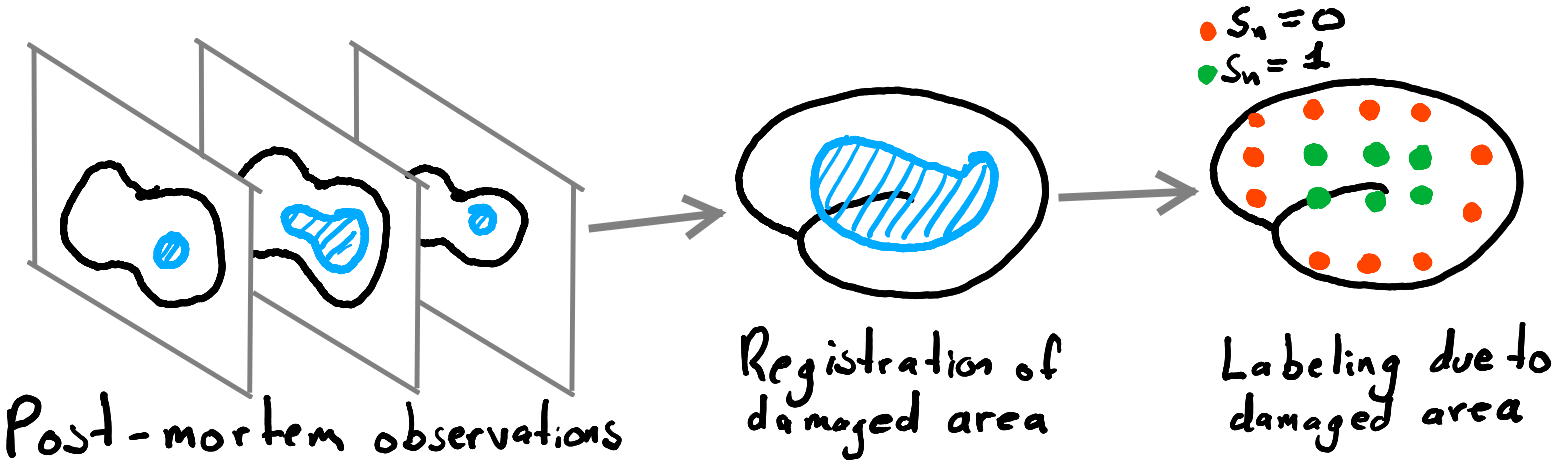
\includegraphics[width=0.8\linewidth]{./img/sketch02_v2}
%\end{figure}

The relation between the current density, $\SA$, and the P-regions is incorporated into the model by adjusting the expected value of $\SA$ depending on whether it is located in a P-region.
%
To be specific, consider,
\begin{equation}
    E\spar{\SA\ppar{t,n}} = 
    \begin{cases}
        \U\ppar{t,k}, & \text{if } n\in R_k \text{ with } 0<k, \\
        0, & \text{otherwise}
    \end{cases}
\end{equation}
%with $\U \in \R^{K\times T}$ a the collection of regional averages. 
%Thus any dipole located on a region with no symptoms is treated as generating only noise with low amplitude.

This assumption can be interpreted as assuming that each pathologic region exhibits a synchronized activity with background noise no larger than the background noise from other regions.
%
Such synchronized activity should be larger than the noise in order to be significant to the model.

The model can be condensed as
\begin{equation}
    \J = \PA \U + \N
\end{equation}
where $\mathbf{U}\in \R^{K\times T}$ and $\mathbf{N}\in \R^{N\times T}$ are independent and satisfy
\begin{equation}
    \text{Var}\ppar{\N_{t,n}} \ll \text{Var}\ppar{\U_{t,k}}.
\end{equation}

The proposed model is driven by the following equations
\begin{align}
    \Y &= \G \ppar{\PA \U + \N} \\
    \N_t &\sim  
    \norm\ppar{0, \gamma_0^2 \id } \\
    \U_t &\sim  
    \norm\ppar{0, \gamma_1^2 \id } 
\end{align}
%where 
%$\Y, \G$ and $L_S = \text{diag}\ppar{S} L$ are given, and
with $\gamma_0^2 \ll \gamma_k^2$.

\section{Proposed Estimator}

The proposed estimator for $\SA$ is derived as a Maximum A Posteriori (MAP) from ().
%
In other words, we want
\begin{align}
    \ppar{ \hat{\U}, \hat{\N} } &=
    %\set{ \hat{\J}, \hat{\ga} } &=
    \argmax_{\U, \N }\,
    %\argmax_{\J, \ga}\,
    \log P\ppar{\ppar{ {\U}, {\N} } \Big| {\Y; \gamma_0, \gamma_2} }
\end{align}
which derives into the following error function
\begin{align}
    F\ppar{ {\U}, {\N};  \gamma_0, \gamma_1} &=
    \frac{1}{2\sigma^2}
    \nnorm{\G L_S \U + \G \N - \Y}_F^2
    \nonumber \\
    &\phantom{=}
    +
    \frac{1}{2\gamma_0^2} \nnorm{\N}_F^2
    +
    \frac{1}{2\gamma_1^2} \nnorm{L_S \U}_F^2
\end{align}
 


 {Maximum A Posteriori (MAP) estimator}
    The iterative minimization of the error function can be interpreted as a multi-scale iterative correction
    \begin{align}
        \hat{\N}^{(i+1)} &= \argmin_{\N} F\ppar{\U^{(i)},\N; \gamma_0, \gamma_1}
        \\
        \hat{\U}^{(i+1)} &= \argmin_{\U} F\ppar{\U,\N^{(i)}; \gamma_0, \gamma_1}
    \end{align}
    These steps have the following closed-form
    \begin{align}
        \hat{\N}^{(i+1)} &=
        \hat{\N}^{(i)}
        -
        \G^T \spar{\G \G^T + \frac{\gamma_0^2}{\sigma^2} \id}^{-1} L_S \ppar{\hat{\U}^{(i)}-\hat{\U}^{(i-1)} }
        \\
        \hat{\U}^{(i+1)} &=
        \hat{\U}^{(i)}
        -
        L_S^T \G^T \spar{\G L_S L_S^T \G^T + \frac{\gamma_1^2}{\sigma^2} \id}^{-1} \ppar{\hat{\N}^{(i)}-\hat{\N}^{(i-1)} }
    \end{align}

\section{Results}

\subsection{Real Data}

The effectiveness of the method is tested using data from an experiment 
of acute ischemic stroke on an animal model, performed by
Pascal [cite].

Posterior to the experiment, the subject is sacrificed.
%
The brain is fragmented in frontal slices for staining with
2, 3, 5 
triphenyltetrazolium (TTC)
to identify the anatomical region damaged by hypoxia\footnote{Lack of oxygen at a cellular level.}, which is also known as the Ischemic Penumbra

The operation of the TTC staining is based on the fact that TTC (white) 
%is a white compound, but it 
is degraded to 1,3,5-triphenyl formazan (TPF, red)
on the presence of dehydrogenases in metabolically active cells.
%
As a result, tissue colored white was affected by necrosis, and tissue colored red was unaffected. 
[cite Wiki?]

%\begin{figure}
%\centering
%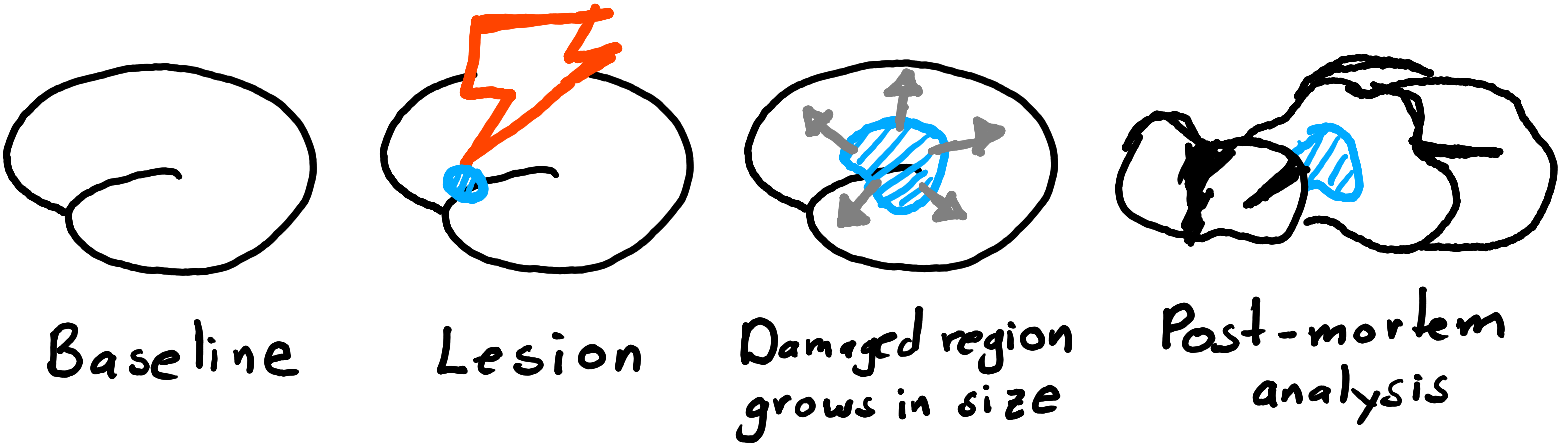
\includegraphics[width=0.8\linewidth]{./img/sketch01_v2}
%%\caption{This figure is temporary and will be replaced}
%\end{figure}

Within the framework of this work, pictures obtained after TTC staining were registered to the template MRI in order to identify the Ischemic Penumbra at the time of sacrifice.
%
This definition is simplistic and doesn't represent a clinical decision.

The active region defined in the section [], $Z$, is determined using the obtained information: a dipole $i$ is labeled as $Z_i=1$ if and only if it is located on the Ischemic Penumbra.



\section{Previous text}





 



 




 


